\section{Auswahl einer Drohne} \label{drone_selection}

Bei der Auswahl der Drohne sind vor allem zwei Bereiche zu betrachten:

\begin{itemize}
	\item Die gesetzlichen Rahmenbedingungen zur Drohne und
	\item Die technischen Anforderungen an die Drohne.
\end{itemize}

Aufgrund der gesetzlichen Auflagen aus Kapitel \ref{drohnen} wurde der Beschluss gefasst, dass die auszuwählende Drohne nur innerhalb von geschlossenen Wohnräumen im privaten Betrieb genutzt werden soll und zudem ein Startgewicht von unter 250g besitzen soll. Um eine studentische Machbarkeitsstudie durchführen zu können, ist eine solche eingeschränkte Anwendungsumgebung ausreichend. 

Die Programmierbarkeit der Drohne gehört zu der wichtigsten technischen Anforderung an die Drohne. Zudem soll sie eine integrierte Kamera aufweisen, die in der Lage ist, einen Videostream zur Laufzeit zur Verarbeitung bereit zu stellen. Hierzu wurden in Kapitel \ref{drohnen} bereits die beiden auf dem Markt verfügbaren Modelle  gegenübergestellt. Eine Wahl kann nur zwischen den beiden Modellen der \textit{Bebop 2} von der Firma Parrot oder der \textit{Tello EDU} Drohne von der Firma Ryze Tech getroffen werden. Die gesetzlichen Auflagen, speziell die Kennzeichnungspflicht, und die daraus abgeleiteten, projektkrelevanten Bedingungen lassen allerdings nur die \textit{Tello EDU} Drohne zu, zudem sie mit vertretbaren Budget erworben werden kann. Des Weiteren wird noch eine Garantie zu präzisem Schweben geboten, was gerade für die Objektdetektion vorteilhaft werden kann. Im Vergleich dazu erscheint die \textit{Parrot Bebop 2} vielmehr als eine Drohne, die für den Einsatz im Außenbereich konzipiert wurde.

---- Unteren Teil in 4.4 ------

Für die Steuerung sowie den Zugriff auf den Videostream bietet die \textit{Tello EDU} ein eigenes WiFi Netz an, zu dem sich das Steuergerät verbinden muss. Die Kommunikation erfolgt über das \textit{UDP} Protokoll\footnote{UDP steht für User Datagram Protocol. Es ist ein Transportprotokoll, welches im Gegensatz zu TCP verbindungslos und nicht zuverlässig ist.} und besteht aus mehreren Kommunikationskanälen: 

\begin{figure}[H]
	\begin{center}
		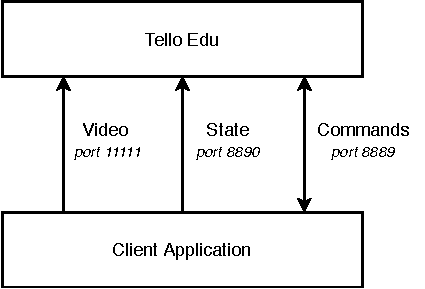
\includegraphics[width=8cm]{Bilder/communication_tello.pdf} 
		\caption{Kommunikationskanäle der Tello EDU Drohne}
		\label{communication_tello}
	\end{center}
\end{figure}

Der Video Stream und der Status der \textit{Tello EDU} werden unidirektional durch die Client Applikation bei der \textit{Tello EDU} abgefragt, wohingegen für das Senden von Befehlen eine bidirektionale Verbindung zum Einsatz kommt. Das liegt daran, dass die \textit{Tello EDU} auf jeden erhaltenen Befehl auch eine Antwort zurücksendet. Es existieren Befehle zur Steuerung und zum Auslesen von Informationen wie zum Beispiel der Geschwindigkeit oder Ladezustand der Batterie. Als Hilfestellung wird zusätzlich ein Beispielprogramm mitgeliefert, in welchem das Senden und Empfangen von Befehlen implementiert wurde \cite{RyzeTech.2018}. 